\documentclass[conference]{IEEEtran}
\IEEEoverridecommandlockouts
% The preceding line is only needed to identify funding in the first footnote. If that is unneeded, please comment it out.
\usepackage{cite}
\usepackage{amsmath,amssymb,amsfonts}
\usepackage{algorithmic}
\usepackage[ruled,norelsize]{algorithm2e}
\usepackage{graphicx}
\usepackage{textcomp}
\usepackage{color}
\usepackage{xcolor}
\usepackage{listings}
\usepackage{booktabs}
\usepackage{soul}
\usepackage{url}

\newcommand{\ttt}[1]{\tt\small{#1}}
\newcommand{\tool}{{\ttt CodeAid}}
\lstset{
	% numbers=left,
	% numberstyle=\tiny,
	% backgroundcolor=\color{light-gray},
	basicstyle=\scriptsize\ttfamily,
	breaklines=true,
	breakatwhitespace=true,
	captionpos=b,
	columns=flexible,
	escapeinside={(*@}{@*)},
	frame=tb,
	framerule=0.6pt,
	% xleftmargin=\parindent,
	% xrightmargin=\parindent,
	language=Java,
	% numbersep=5pt,
	showstringspaces=false
}
\newcommand{\explanation}[1]{
	\parbox{0.45\textwidth}{
		\rule{0.4\textwidth}{0.1pt}
		\vspace*{0.5em} \\
		{#1}
	}
}

\def\BibTeX{{\rm B\kern-.05em{\sc i\kern-.025em b}\kern-.08em
    T\kern-.1667em\lower.7ex\hbox{E}\kern-.125emX}}
\begin{document}

\newcommand\todo[1]{\textcolor{red}{TODO: #1}}

\makeatletter
\newcommand{\removelatexerror}{\let\@latex@error\@gobble}
\makeatother


\title{CodeAid: Recommending Related Code
%	\\
%{\footnotesize \textsuperscript{*}Note: Sub-titles are not captured in Xplore and
%should not be used}
%\thanks{Identify applicable funding agency here. If none, delete this.}
}

%\author{\IEEEauthorblockN{1\textsuperscript{st} Given Name Surname}
%\IEEEauthorblockA{\textit{dept. name of organization (of Aff.)} \\
%\textit{name of organization (of Aff.)}\\
%City, Country \\
%email address}
%\and
%\IEEEauthorblockN{2\textsuperscript{nd} Given Name Surname}
%\IEEEauthorblockA{\textit{dept. name of organization (of Aff.)} \\
%\textit{name of organization (of Aff.)}\\
%City, Country \\
%email address}
%\and
%\IEEEauthorblockN{3\textsuperscript{rd} Given Name Surname}
%\IEEEauthorblockA{\textit{dept. name of organization (of Aff.)} \\
%\textit{name of organization (of Aff.)}\\
%City, Country \\
%email address}
%\and
%\IEEEauthorblockN{4\textsuperscript{th} Given Name Surname}
%\IEEEauthorblockA{\textit{dept. name of organization (of Aff.)} \\
%\textit{name of organization (of Aff.)}\\
%City, Country \\
%email address}
%\and
%\IEEEauthorblockN{5\textsuperscript{th} Given Name Surname}
%\IEEEauthorblockA{\textit{dept. name of organization (of Aff.)} \\
%\textit{name of organization (of Aff.)}\\
%City, Country \\
%email address}
%\and
%\IEEEauthorblockN{6\textsuperscript{th} Given Name Surname}
%\IEEEauthorblockA{\textit{dept. name of organization (of Aff.)} \\
%\textit{name of organization (of Aff.)}\\
%City, Country \\
%email address}
%}

\maketitle

\begin{abstract}
Finding similar code for a given code query can help programmers
detect situations that they had overlooked, or that they did not know
how to solve. Most code-to-code search tools aim at finding
syntactically or semantically similar code given some code of
interest. We take a different approach to code-to-code search: we want
to recommend relevant {\em auxiliary} or {\em complementary}
code. Such relevant code is not semantically similar to the code
query, but it is may be important, because it works together with the
given code to accomplish a complete or related functionality.

In this paper, we describe a code recommendation technique, CodeAid, that returns
relevant code fragments in our search code base related to a code query. We
use GitHub Java projects as our search code base. Given a source code method,
we use a code clone detection tool to detect all its similar
counterparts from different GitHub files, then recommend other related
methods, based on co-occurrence statistics.

In order to evaluate the performance of CodeAid, we use Stack Overflow
(SO) Java code snippets as queries, and measure the precision of the
retrieved related methods. We gathered a query code base of 21,207 SO
Java code snippets. For 11,110 of these, CodeAid returns their related
code fragments. Then we manually evaluate the relevance of the
recommended GitHub code. Using this methodology, CodeAid has a
precision of 75.6\%. We also categorize the relationship between the
recommended code and the SO query snippet, in order to shed light on
how CodeAid can be useful in practice.

\end{abstract}

\begin{IEEEkeywords}
code recommendation, related code, code search, mining software repositories
\end{IEEEkeywords}

\section{Introduction}
\label{sec:intro}

Over the past decade, code search has emerged as an interesting, but
challenging, topic to both industry and research communities. Various code search
techniques have been proposed in the
literature~\cite{bajracharya2009sourcerer,reiss2009semantics,lazzarini2009applying,mcmillan2012exemplar}, and
some search code engines have been implemented and are, or were, publicly
available~\cite{googlesearch, github,codase,krugle,ohloh,searchcode}. All
of these code search engines take some specification as input (a
query, a code fragment, or a test) and retrieve pieces of code that try
to match that specification.

% motivation example

This work addresses the code search problem from a different angle. Consider
the following scenario. A programmer is implementing a Java method for
file decompression; this method gets as input the path to a zip file
 unpacks all files within the zip into a target directory, as shown in 
 Listing~\ref{lst:mot-query}. This piece of code is sufficient for 
 a simple program task of unpacking a zip file. However, in pratice, the programmer 
 may undertake a more complex programming task where unzipping a file is a small,
 integral part. Therefore, the programmer may also want to know what else may be
related to this functionality. %, in case they will also need that in the future. 
The programmer may also want to have a comprehensive understanding of the collection of related
functions for zip file manipulation, in general. If an additional
functionality often co-occurs with unzipping, the programmer may want to add it
to her own project as needed. Listing \ref{lst:mot-related} shosws an example of this kind of additional 
functionalities---a method that zips a list of files from a folder into the target zip file. Unzipping
and zipping are two kinds of file manipulation in the opposite direction. 
Though these two functions work independently, they are often implemented together in a codebase to facilitate
possible needs from any direction. We consider the zip method and the unzip method {\em related} to each other, or {\em complementary code fragement}, to be more specifically.

\begin{figure*}[!t]
\begin{minipage}[t]{0.5\linewidth}
\begin{lstlisting}[style=MyJavaSmallStyle, caption={Query code\todo{Simply listing 1 to a similar length as listing 2}}, label={lst:mot-query}]
public static boolean unpackZip(String path, String zipname, String targetDirectory) {
	InputStream is;
	ZipInputStream zis;
	try {
		String filename;
		is = new FileInputStream(path + zipname);
		zis = new ZipInputStream(new BufferedInputStream(is));
		ZipEntry ze;
		byte[] buffer = new byte[1024];
		int count;

		while ((ze = zis.getNextEntry()) != null) {
			filename = ze.getName();

			if (ze.isDirectory()) {
				File fmd = new File(targetDirectory + filename);
				fmd.mkdirs();
				continue;
			}

			FileOutputStream fout = new FileOutputStream(targetDirectory + filename);

			while ((count = zis.read(buffer)) != -1) {
				fout.write(buffer, 0, count);
			}

			fout.close();
			zis.closeEntry();
		}

		zis.close();
	} catch (IOException e) {
		e.printStackTrace();
		return false;
	}

	return true;
}
\end{lstlisting}
\end{minipage}
%
\begin{minipage}[t]{0.5\linewidth}
\begin{lstlisting}[style=MyJavaSmallStyle, caption={Recommended related code}, label={lst:mot-related}]
public static void zip(String baseFolder, List<File> files, String zipFile) {
	try  {
		BufferedInputStream origin = null;
		FileOutputStream dest = new FileOutputStream(zipFile);

		ZipOutputStream out = new ZipOutputStream(new BufferedOutputStream(dest));
		byte data[] = new byte[BUFFER];

		for (File file : files) {
			FileInputStream fi = new FileInputStream(file);
			origin = new BufferedInputStream(fi, BUFFER);
			String relativeFileName = file.getAbsolutePath().replace(baseFolder + File.separator , """");
			ZipEntry entry = new ZipEntry(relativeFileName);
			out.putNextEntry(entry);
			int count;
			while ((count = origin.read(data, 0, BUFFER)) != -1) {
				out.write(data, 0, count);
			}
			origin.close();
		}

		out.close();
	} catch(Exception e) {
		e.printStackTrace();
	}

}
\end{lstlisting}
\end{minipage}
\end{figure*}
% code search and code completion

Code-to-code search engines could potentially be used to get code
recommendations for our unzipping example. For example, code-to-code search tools
~\cite{kim2018Facoy, krugle, searchcode} could take the code snippet
as query and retrieve similar code snippets from their code
corpora. However, such code-to-code search tools aim at finding
similar code, not extra functionality, so they retrieve several
versions of unzipping files. 

Pattern-based code completion tools~\cite{nguyen2009groum,
  nguyen2012grapacc} also recommend completing code for a given code
query. They do so by mining common API usage patterns from a large
code corpus. For a given partial snippet as query, if it matches a
prefix of a mined pattern, the tool recommends the rest of the pattern
for completion. Again, such tools only work for the mined patterns;
that is, they do not recommend code outside the mined patterns.

For both code search engines and pattern-based code completion tools,
the retrieved code snippets may have extra lines of code with more
functionality, but they are not designed to search for commonly used
additional code.

The goal of our work is to support the search needs shown in Listings
\ref{lst:mot-query} and \ref{lst:mot-related}. In this paper, we
describe {\tool}, a recommendation engine for related code. Given a
code snippet as input query and a large corpus of code containing
millions of code fragments, {\tool} returns a set of recommended code
fragments such that:
\begin{itemize}
	\item the recommended code fragments co-occur with similar counterparts of the input query.
	\item the recommended code fragments are ranked by their
          relevance as complements to the input query.
\end{itemize}


For the time being, we focus on method-level code fragments written in
Java. Both the query snippet and the recommended related code
fragments are Java methods. {\tool} works by first tokenizing the
query and all methods in the code corpus. It then uses token
similarity to detect similar counterparts to the query in the code
corpus. We delegate this process to a clone detection tool,
SourcererCC~\cite{sajnani2016sourcerercc}. Finally, {\tool} recognizes
other methods which co-occur with these similar counterparts as
candidate related methods.

% advantages of CodeAid
{\tool} has the following properties:
\begin{itemize}
	\item It retieves functionality groups, which the user may want to implement together with the input query.
	\item It has a clustering algorithm on top of co-occurrence to provide ranking.
	\item It is not restricted to any programming language. The Java parser is only used to chunk the file into methods, it can be replaced by the parser from any languages as needed.
	\item It has flexible granularity level. We can chunk the files into blocks of any size. All similarity comparison processes are token-based, which means as long as we have the token list representing the block, it does not matter what size the block is.
	\item It is fast enough to be used in real time. The most
          time-consuming part is similar code detection. However,
          generating the indexes is a one-time task and can be done
          before any query is processed.	
\end{itemize}

In order to evaluate {\tool}, we use two datasets: (1) a query dataset
consisting of 21,207 Java code snippets collected from Stack Overflow
(SO), and (2) a large Java code base consisting of 50,826 projects which 
have at least five starts collected from GitHub, with over 5.8M distinct 
Java files. We then run each query in the query dataset through {\tool} 
and collect the recommended fragments coming from the code base. 
We present both a quantitative and qualitative analysis of the results.
We build a chrome extension for Stack Overflow as a proof of concept and also to help with the qualitative evaluation.

The rest of the paper is organized as follows: Section
\ref{sec:approach}, we describe the algorithm {\tool} uses to generate
recommendations. In Section \ref{sec:eval}, we manually analyze how
relevant {\tool} recommendations are, and what kinds of relevance they
provide. We also compare {\tool} results with those from code search
engines in this section. The use scenario of the chrome extension is introduced in Section \ref{sec:chrome}. Section \ref{sec:related} presents the
related work. Finally, Section \ref{sec:conclude} concludes the paper.

\section{Data Collection Approach}
\label{sec:approach}
Our approach takes a code fragment as input and searches a code corpus to identify related code fragments. Given a user-selected code fragment, we first detect its similar methods in the corpus based on syntactic similarity. Then we trace back to the containing files of these similar methods and identifies other co-occurring methods in these files. Among these co-occurring methods, we further measure each method's similarity to methods in other files, and cluster similar methods. Then we rank co-occurring methods based on the size of cluster it centers. Figure~\ref{fig:pipeline} describes the pipeline of finding commonly co-occurring code fragments in {\tool}. 


\begin{figure}
	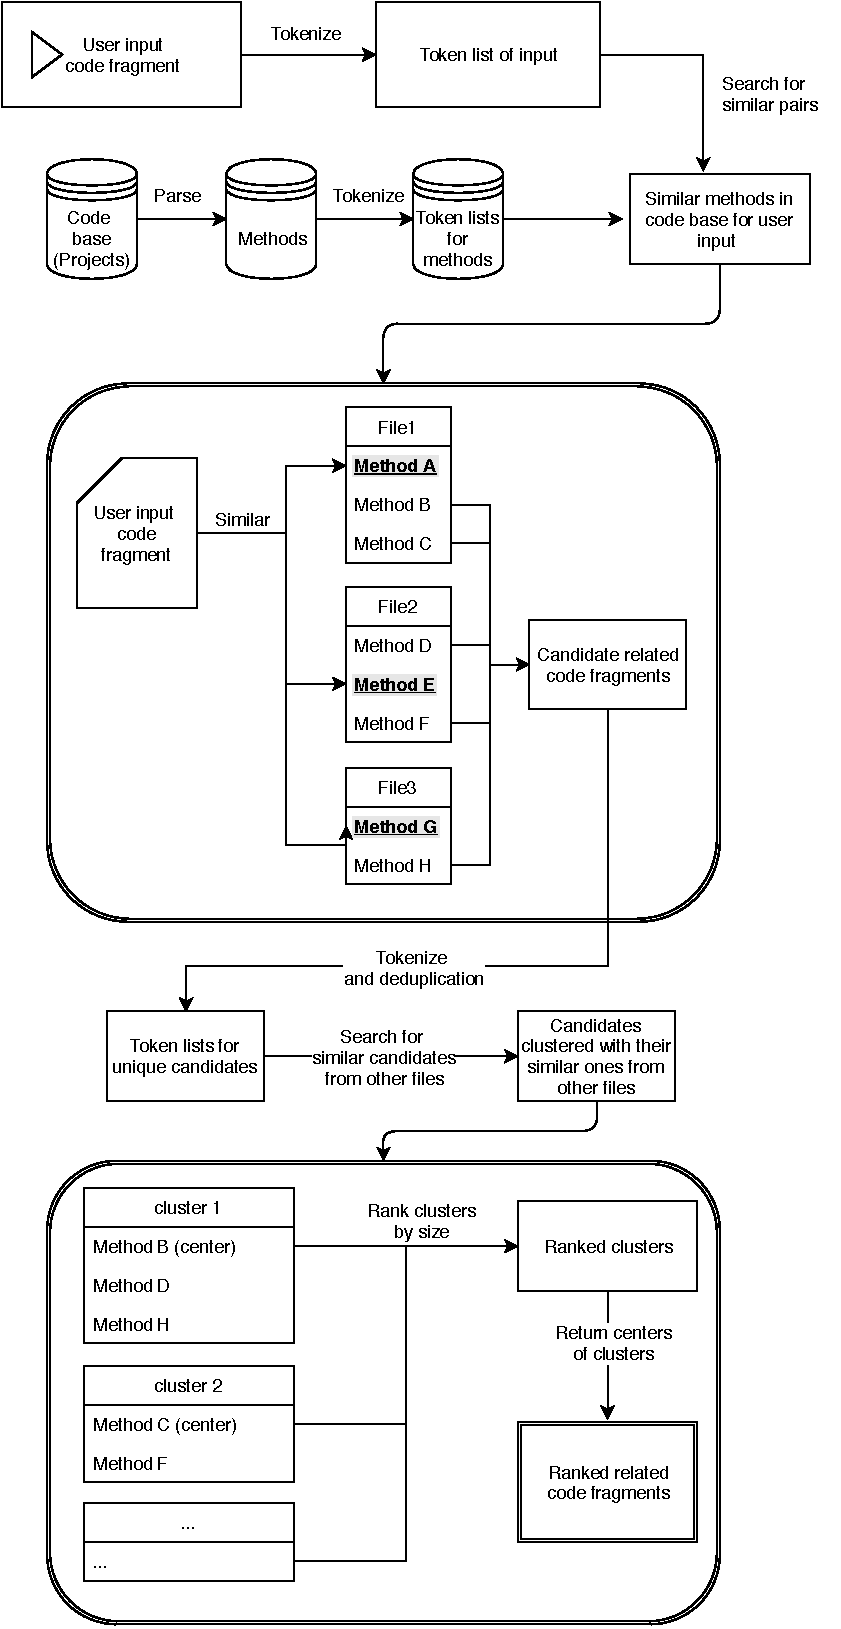
\includegraphics[width=\linewidth]{figures/pipeline.pdf}
	\caption{The pipeline of collecting commonly co-occurring methods}
	\label{fig:pipeline}
\end{figure}

\subsection{Retrieve similar methods}
\subsubsection{Parse a code corpus}
We focus on method-level code fragments written in Java in this work. We parse all Java source files to abstract syntax trees (ASTs) and traverse the ASTs to extract all defined methods. Note that the approach is not limited to any programming language. We can switch to any other language by using its particular parser. We use the phrases code fragments and methods interchangeably in the paper.

\subsubsection{Tokenization}
Tokenization is the process of transforming source code into a bag of words. Tokenization starts from removing comments, spaces, tabs and other special characters. Then it identifies distinct tokens and count their frequencies. For each method, the result of tokenization is formatted as a list of tuples such as {\ttt (token, freq)}, where the first element is a token in the method and the second element refers to the token occurrence in the method.

We tokenize both the input code fragment and all methods in the code corpus, in preparation for the next step of finding similar pairs.

\subsubsection{Search for similar methods}
For the input code fragment, we retrieve its similar counterparts from the code corpus using a token-based clone detection tool called SoucererCC~\cite{sajnani2016sourcerercc}. By evaluating the scalability, execution time, recall and precision of SourcererCC, and comparing it to publicly available and state-of-the-art tools, SourcererCC has been shown to have both high recall and precision, and is able to scale to a large repository using a standard workstation. All of the above make SourcererCC a good candidate for building our code recommendation engine. 

%Given a similarity threshold, SoucererCC takes three steps to detect clones. First, it tokenizes a code snippet to a set of tokens. This tokenization step removes comments, whitespaces, and special characters and also counts the frequency of individual tokens. Second, SoucererCC creates a partial index of each snippet by selecting and indexing a subset of tokens based on heuristics, and builds an inverted index mapping between tokens and code snippets. Finally, SoucererCC iterates through all snippets and finds candidate clones of each snippet by querying the inverted index mapping. After retrieving the candidates, SoucererCC uses another heuristic which exploits ordering of the tokens in a snippet to verify the candidates and locate the clones. 
We use 70\% similarity threshold, because it yields the best precision and recall on multiple clone benchmarks~\cite{sajnani2016sourcerercc}. SourcererCC takes the token lists of the input code fragment and all methods in the code corpus, and returns the similar methods to the input in the code corpus. As shown in Figure \ref{fig:pipeline}, the user input has three similar counterparts in our code corpus, which are {\ttt Method A} in {\ttt File1}, {\ttt Method E} in {\ttt File2}, and {\ttt Method G} in {\ttt File3}.

\subsection{Identify co-occurring code fragments}
Given those similar code fragments identified in the previous step, we trace back to the files that contain these similar counterparts and identify co-occurring methods in the same file as a potentially related code fragment. Algorithm~\ref{alg: co-occur} gives a more formal description of the process.

\begin{figure}[h]
		
 \removelatexerror
\begin{algorithm}[H]
	\label{alg: co-occur}
	\caption{Identify co-occurring code fragments}
	\KwData{similar methods}
	\KwResult{co-occurring methods}
	initialize $resultList$\;
	\For{$m_s$ in $similarMethods$}
	{
		$ghFiles$ = traceGitHubFiles(method) \;
		\For{$f$ in $ghFiles$}
		{
			$methodsInFile$ = parse($f$)\;
			\For{$m_f$ in $methodsInFile$}
			{
				\If {$m_f$ is not $m_s$}
				{
					$resultList$.add($m_f$) \;
				}
			}
		} 
	}
\end{algorithm}
\end{figure}

{\ttt Method A, E, G} are the three similar methods detected by SourcererCC. {\ttt File 1, 2, 3} are the three GitHub files contain these similar methods respectively. 
{\ttt File1} also contains {\ttt Method B, C}, {\ttt File2} has another two methods {\ttt Method D, F}, and {\ttt Method H} is in {\ttt File3}. Therefore, {\ttt Method B, C, D, F, H} will be returned as co-occurring methods by Algorithm~\ref{alg: co-occur}.

\subsection{Clustering and Ranking}
\subsubsection{Cluster co-occurring code fragments}
We further get the token lists for those co-occurring methods identified in the previous step and remove duplicate methods. Duplication is defined as same token lists. In order to detect common co-occurring code fragments, we cluster the remaining unique oc-occurring methods
based on their token similarity. Given each method, we compute its similarity to other methods from different GitHub files. Each method will serve as the center of a cluster, we browse among other methods from different files and add similar methods to the current cluster. Algorithm~\ref{alg: clustering} describes the process.

\begin{figure}[h]
	\removelatexerror
	\begin{algorithm}[H]
		\label{alg: clustering}
		\caption{Clustering candidate related code fragments}
		\KwData{$n$ candidate related methods}
		\KwResult{clustered candidate methods}
		initialize $clusters$ = $\{X_1, X_2,..., X_n\}$\;
		\For{$m_i$ in $candidateMethods$}
		{
			$X_i$.add($m_i$) \;
			\For{$m_j$ in $candidateMethods$}
			{
				\If {$m_i$ and $m_j$ do not come from the same file}
				{
					\If {tokenSimilarity($m_i$, $m_j$) $>$ 0.7)}
					{
						$X_i$.add($m_j$);
					}
				}
			} 
		}
	\end{algorithm}
\end{figure}

For the co-occurring methods pool, {\ttt Method B, C, D, F, H}, each method will be the center of a cluster. For {\ttt Method B}, we compute token similarity with {\ttt Method D, F, H} and get two similar ones, {\ttt Method D, H}, so we add these two similar methods to the cluster, resulting in cluster size being three. Similarly, we add {\ttt Method F} to the cluster centered by {\ttt Method C} and get a cluster with size two.

\subsubsection{Screen and rank clusters by size}
After getting the candidate clusters, we keep only clusters with size being at least two. This means the center of the cluster has occurred at least twice among the GitHub files.
We rank the remaining clusters by size and return the cluster centers as our final list of commonly co-occurring code fragments with ranking. If two clusters have the same size, we will order them by the line number distance between the cluster center and the original counterparts of the query (e.g. {\ttt Method C, A}), in ascending order. We will return {\ttt Method B} first, and then {\ttt Method C}, as our common co-occurring code fragments.
\section{Data Collection}
\label{sec:dataset}
We apply our approach to Stack Overflow (SO) and GitHub. We use code snippets in SO as the pool of user-selected examples and use Java projects in GitHub as our code corpus to search from. We choose these two datasets not only because of their popularity within the programming community, but also because they are part of a larger system of software production. The same users that rely on the hosting and management characteristics of GitHub often have difficulties and need help on the implementation of their computer programs, seek support on SO for their specific problems, or hints of solutions from ones with a degree of similarity, and return to GitHub to apply the knowledge acquired. Previous work have shown that developers often copy and paste code snippets from Stack Overflow to their GitHub projects and make adaptations as needed~\cite{yang2017stack, an2017stack, wu2018developers, zhang2019analyzing}. Our approach will facilicate such opportunistic code reuse process when developers browse code snippets in Stack Overflow. The use scenario will be: when a user is interested in a code snippet in SO, CodeAid recommends related code fragments from GitHub, showing what other code she may also want to investigate and integrate into her own project. \todo{Di, if you have implemented the Chrome extension we discussed before, it would be great to add a screenshot of the Chrome extension here.} 


\subsection{GitHub}
We downloaded Java projects on GitHub by querying GHTorrent. GHTorrent is a scalable, offline mirror of data offered through the Github REST API, available to the research community as a service~\cite{gousios2012ghtorrent}. It provides access to all the metadata of GitHub projects, e.g., the number of stars and commiters, main programming languages in a project, etc. Since GitHub has many toy projects that do not adequately reflect software engineering practices~\cite{kalliamvakou2014promises}, we only consider GitHub projects that have at least five stars. To account for internal duplication in GitHub~\cite{lopes2017dejavu}, we choose non-fork projects only and further remove duplicated GitHub files using the same file hashing method as in~\cite{lopes2017dejavu}, since such file duplication may skew our analysis. As a result, we download 50,826 non-forked Java repositories with at least five stars from GitTorrent. After deduplication, 5,825,727 distinct Java files remain.%\todo{fix the citations.}


\subsection{Stack Overflow}
From the SO dump taken in October 2016, we extract 312,219 answer posts that have java or android tags and also contain code snippets in the {\ttt <code>} markdown. We consider code snippets in answer posts only, since snippets in question posts are rarely used as examples. Since SO snippets are often free-standing statements with low parsable rates, we used a customized pre-processor before tokenization. We add dummy class and method definitions, and semicolons after statements, as needed. For snippets contain multiple methods, we chunk them into individual ones. We keep only parsable SO snippets after pre-processing. Prior work finds that larger SO snippets have more meaningful clones in GitHub~\cite{yang2017stack}. Hence, we choose to study SO examples with no less than 50 tokens after tokenization. We also remove duplicated examples within SO.%\todo{fix the citations}

\subsection{Result for similar code detection}
We run SoucererCC to find all similar pairs between SO and GitHub. As a result, we get 21,207 distinct SO methods that have one or more similar code fragments in GitHub. \todo{talk more about the running enviroment and how long it takes to process the dataset, in order to show the construction effort.}

\subsection{Result for candidate related methods}
Within the 21,207 groups of SO snippet with GitHub files which contain similar methods to the SO snippet, we extract all co-occurred methods from these GitHub files and treat them as candidate related code fragments. Then for each candidate in each GitHub file, we retrieve its similar counterparts from other files. As a result, we get the co-occurred methods as our candidate related code fragments and for each candidate we also have the frequency of its similar counterparts. Not all groups have candidate methods and not all candidates have similar counterparts in other files, we have 11,110 SO snippets whose candidate related methods do have similar counterparts in other files, that can be taken as the candidate appears more than one files and we take this as a stronger signal for recommendation and only focus on these 11,110 groups from then on. Inside each group, we order the candidates by the number of similar counterparts and returned the ordered list as the final recommendation of related code fragments to the user. \todo{I suggest to add some statistics of these identified related methods. For example, how big are these methods in terms of LOC? For those SO snippets with related GitHub examples, how many related examples they have? Maybe we can also analyze the domains of SO snippets with SO, since I remember you mentioned that a lot of them are from Android.}

\todo{We also discussed that it is possible to recommend related code examples in another SO post if code snippets in two SO posts map to the same GitHub file. Would you still like to mention it here?}

\section{Evaluation}
\label{sec:Evaluation}
In this section, we describe the design of the assessment scenarios for \tool\ and report the evaluation results. Specifically, our experiments aim to address the following research questions:
\begin{itemize}
	\item RQ1: Are the code fragments recommended by \tool\ related to the query?
	\item RQ2: What kinds of related code fragments do \tool\ recommend?
	\item RQ3: Can we get the recommended related code fragments from code search engines?
\end{itemize}

\subsection{Manual analysis and categorization}
We randomly select 30 SO snippets with its recommended related code fragments, and manually examine whether the recommended code fragments are related to the SO input or not, and categorize why we call the relationship a relevant one.

We use $Precision@k$ metric to evaluate \tool\  which is defined as follows:
\begin{equation}
Precision@k = \frac{1}{N}\sum_{i=1}^{N}\tfrac{\left | relevant_{i,k} \right |}{k}
\end{equation}
where $\left | relevant_{i,k} \right |$ represents the number of positive related results in the top $k$ results for query $i$, $N$ is the number queries we evaluate, which is $30$. $k$ is the number of top results we examine, here we use $k=1$ and $k=3$.

\tool\ achieves 80\% and 78.9\% for $Precision@1$ and $Precision@3$ respectively. That is to say, for the 30 top 1 recommended results, 24 of them are manual examined as related, for the 90 top 3 recommended resutls, 71 of them are related.

We find the following types of relevance in our sample set.
\begin{itemize}
	\item A complementary method which adds more functionality
	\item A supplmentary method that help with or get help from the query 
	\item A different implementation for the query	
\end{itemize}

\begin{table}
	\begin{center}
		\begin{tabular}{ c|c|c } 
			Category & Top 1 & Top 3 \\\hline
			Complementary method &  12 & 33\\\hline 
			Supplementary method &  11 & 31 \\ \hline
			Different implementation &  1 & 4 \\ \hline
			Not related &6 & 19
		\end{tabular}		
	\end{center}
	\caption{Categorization of related methods}
	\label{tab:categorization}
\end{table}
	
	

\subsubsection{Complementary method} In this category, the query code can function alone, but the recommended related method provides extra functionality to the query code and will further complete the user class. As shown in the Table ~\ref{tab:compl-examples}, \tool\ recommends \texttt{Zip} function when the user implements \texttt{Unzip}. Similarly, \texttt{Decrypt} function for \texttt{Encrypt} and \texttt{onPause} function for \texttt{onCreate}. The two methods do not have any direct function call association between them, but they complete each other with extra functionality and are often implemented together in real-life scenarios. 

\subsubsection{Supplementary method} The recommended related code serves as a helper function to the query, or vice versa. One may make function call to the other. For example the \texttt{Merge} function for \texttt{Sort}. \texttt{Sort} calls \texttt{Merge} as a helper function and cannot achieve functionality without it. Also in our second example Table ~\ref{tab:suppl-examples}, our recommended related code \texttt{loadDrawable} calls \texttt{queueJob} inside its method body. There is another related method being recommended together, which is shown below \ref{lst:part2}. This code is also called by \texttt{loadDrawable}, the related methods give the user a broader picture of the whole class,point to a higher level of functionality the user may want to implement, and also direct the user to the most-frequently used higher level functionality and its auxiliaries.
\begin{lstlisting}[caption={Recommended code \#2}, label={lst:part2}]
public static Drawable getDrawableFromCache(String url) {
	if (DrawableManager.cache.containsKey(url)) {
		return DrawableManager.cache.get(url);
	}
	
	return null;
}	
\end{lstlisting}

\subsection{Different implementation} This category represents those recommended related methods which have similar functionality to the query code. The recommended result provide an alternative, or a more detailed or extended implementation for the functionality. As shown in Table ~\ref{tab:diff-examples}, both of the methods implement sorting values in a \texttt{Map}, the query store the map entries in a \texttt{SortedSet}, while the recommended code uses \texttt{LinkedList}, and shows how to iterate a \texttt{Map}. For the \texttt{encryt} in Table ~\ref{tab:compl-examples}, \tool\ also recommended an alternative implementation with \texttt{String} inputs, as shown in Listing ~\ref{lst:encryt}.


\begin{lstlisting}[caption={different implementation for \texttt{encrypt}}, label={lst:encryt}]
public static String encrypt(final String password, String message) throws GeneralSecurityException {
	try {
		final SecretKeySpec key = generateKey(password);
		log("message", message);
		byte[] cipherText = encrypt(key, ivBytes, message.getBytes(CHARSET));
		//NO_WRAP is important as was getting \n at the end
		String encoded = String.valueOf(
			Base64.encodeToString(cipherText, Base64.NO_PADDING ));
		log("Base64.NO_WRAP", encoded);
		return encoded;
	} catch (UnsupportedEncodingException e) {
		if (DEBUG_LOG_ENABLED)
			Log.e(TAG, "UnsupportedEncodingException ", e);
		throw new GeneralSecurityException(e);
	}
}
\end{lstlisting}

% Set listing style for table
\lstset{
	frame=none,
    aboveskip=0pt,
    belowskip=0pt,
    basicstyle=\tiny\ttfamily,
}
\begin{table*}\scriptsize
\caption{Complementary code examples}
\label{tab:compl-examples}

\setlength{\tabcolsep}{0.01\textwidth}
\begin{tabular}{@{}p{0.49\textwidth}p{0.49\textwidth}@{}}
\toprule
Query Code Snippet & Recommended Related Code \\
\midrule



\begin{lstlisting}
public static boolean unpackZip(String path, String zipname, String targetDirectory) {
	InputStream is;
	ZipInputStream zis;
	try {
		String filename;
		is = new FileInputStream(path + zipname);
		zis = new ZipInputStream(new BufferedInputStream(is));
		ZipEntry ze;
		byte[] buffer = new byte[1024];
		int count;

		while ((ze = zis.getNextEntry()) != null) {
			filename = ze.getName();

			if (ze.isDirectory()) {
				File fmd = new File(targetDirectory + filename);
				fmd.mkdirs();
				continue;
			}

			FileOutputStream fout = new FileOutputStream(targetDirectory + filename);

			while ((count = zis.read(buffer)) != -1) {
				fout.write(buffer, 0, count);
			}

			fout.close();
			zis.closeEntry();
		}

		zis.close();
	} catch (IOException e) {
		e.printStackTrace();
		return false;
	}

	return true;
}
\end{lstlisting}


&
\begin{lstlisting}
public static void zip(String baseFolder, List<File> files, String zipFile) {
	try  {
		BufferedInputStream origin = null;
		FileOutputStream dest = new FileOutputStream(zipFile);

		ZipOutputStream out = new ZipOutputStream(new BufferedOutputStream(dest));
		byte data[] = new byte[BUFFER];

		for (File file : files) {
			FileInputStream fi = new FileInputStream(file);
			origin = new BufferedInputStream(fi, BUFFER);
			String relativeFileName = file.getAbsolutePath().replace(baseFolder + File.separator , """");
			ZipEntry entry = new ZipEntry(relativeFileName);
			out.putNextEntry(entry);
			int count;
			while ((count = origin.read(data, 0, BUFFER)) != -1) {
				out.write(data, 0, count);
			}
			origin.close();
		}

		out.close();
	} catch(Exception e) {
		e.printStackTrace();
	}

}
\end{lstlisting}
\vspace*{1em}
\explanation{
    \emph{Example A: Complementary method}
    \begin{itemize}
        \item The query snippet implements unzip a folder in Java.
        \item The recommended related method implements zip a folder. These two methods can function independently, but often implemented together to get a stronger ability for folder manipulation.
    \end{itemize}
}

\\

\bottomrule

\begin{lstlisting}
public static byte[] encrypt(final SecretKeySpec key, final byte[] iv, final byte[] message)
throws GeneralSecurityException {
	final Cipher cipher = Cipher.getInstance(AES_MODE);
	IvParameterSpec ivSpec = new IvParameterSpec(iv);
	cipher.init(Cipher.ENCRYPT_MODE, key, ivSpec);
	byte[] cipherText = cipher.doFinal(message);

	log(""cipherText"", cipherText);

	return cipherText;
}
\end{lstlisting}


&
\begin{lstlisting}
public static byte[] decrypt(final SecretKeySpec key, final byte[] iv, final byte[] decodedCipherText)
throws GeneralSecurityException {
	final Cipher cipher = Cipher.getInstance(AES_MODE);
	IvParameterSpec ivSpec = new IvParameterSpec(iv);
	cipher.init(Cipher.DECRYPT_MODE, key, ivSpec);
	byte[] decryptedBytes = cipher.doFinal(decodedCipherText);

	log(""decryptedBytes"", decryptedBytes);

	return decryptedBytes;
}
\end{lstlisting}

\vspace*{1em}
\explanation{
	\emph{Example B: Complementary method}
	\begin{itemize}
		\item The query snippet implements \texttt{encrypt} functionality for an byte array.
		\item The recommended related method decrypts a decoded byte array. 
	\end{itemize}
}

\\

\bottomrule

\begin{lstlisting}
@Override
public void onCreate(Bundle savedInstanceState) {
	super.onCreate(savedInstanceState);
	setContentView(R.layout.main);
	preferred = (TextView)findViewById(R.id.preferred);
	orientation = (TextView)findViewById(R.id.orientation);
	mgr = (SensorManager) this.getSystemService(SENSOR_SERVICE);
	accel = mgr.getDefaultSensor(Sensor.TYPE_ACCELEROMETER);
	compass = mgr.getDefaultSensor(Sensor.TYPE_MAGNETIC_FIELD);
	orient = mgr.getDefaultSensor(Sensor.TYPE_ORIENTATION);
	WindowManager window = (WindowManager)
	this.getSystemService(WINDOW_SERVICE);
	int apiLevel = Integer.parseInt(Build.VERSION.SDK);
	if(apiLevel <8) {
		mRotation = window.getDefaultDisplay().getOrientation();
	}
	else {
		mRotation = window.getDefaultDisplay().getRotation();
	}
	}
\end{lstlisting}

&
\begin{lstlisting}
@Override
protected void onPause() {
	mgr.unregisterListener(this, accel);
	mgr.unregisterListener(this, compass);
	mgr.unregisterListener(this, orient);
	super.onPause();
}
\end{lstlisting}

\vspace*{1em}
\explanation{
	\emph{Example C: Complementary method}
	\begin{itemize}
		\item The query snippet implements \texttt{onCreate} functionality for an \texttt{Android} activity.
		\item The recommended related method implements \texttt{onPause} which does not have direct function call with the query snippet, but adds extra functionality to the activity. 
	\end{itemize}
}

\\

\bottomrule
\end{tabular}
\end{table*}

\begin{table*}\scriptsize
	\caption{Supplementary code examples}
	\label{tab:suppl-examples}
	
	\setlength{\tabcolsep}{0.01\textwidth}
	\begin{tabular}{@{}p{0.49\textwidth}p{0.49\textwidth}@{}}
		\toprule
		Query Code Snippet & Recommended Related Code \\
		\midrule
		

\begin{lstlisting}
private void queueJob(final String url, final ImageView imageView,final Drawable placeholder) {
	/* Create handler in UI thread. */
	final Handler handler = new Handler() {
	@Override
	public void handleMessage(Message msg) {
		String tag = mImageViews.get(imageView);
			if (tag != null && tag.equals(url)) {
				if (imageView.isShown())
					if (msg.obj != null) {
						imageView.setImageDrawable((Drawable) msg.obj);
					} else {
					imageView.setImageDrawable(placeholder);
					//Log.d(null, "fail " + url);
					}
				}
			}
	};

	mThreadPool.submit(new Runnable() {
		@Override
		public void run() {
			final Drawable bmp = downloadDrawable(url);
			// if the view is not visible anymore, the image will be ready for next time in cache
			if (imageView.isShown())
			{
				Message message = Message.obtain();
				message.obj = bmp;
				//Log.d(null, "Item downloaded: " + url);

				handler.sendMessage(message);
			}
		}
	});
}
\end{lstlisting}


&


\begin{lstlisting}
public void loadDrawable(final String url, final ImageView imageView) {
	imageViews.put(imageView, url);
	Drawable drawable = getDrawableFromCache(url);
	// check in UI thread, so no concurrency issues
	if (drawable != null) {
		Log.d(null, "Item loaded from cache: " + url);
		imageView.setImageDrawable(drawable);
	} else {
		imageView.setImageDrawable(placeholder);
		queueJob(url, imageView);
	}
}
\end{lstlisting}

\vspace*{1em}
\explanation{
	\emph{Example D: Supplementary method}
	\begin{itemize}
		\item The recommended related method calls the query snippet within its method body. It is a higher-level funtionality to the query.
	\end{itemize}
}

\\


\bottomrule


\begin{lstlisting}
@Override
protected void onLayout(boolean changed, int l, int t, int r, int b) {
	final int count = getChildCount();
	for (int i = 0; i < count; i++) {
		View child = getChildAt(i);
		LayoutParams lp = (LayoutParams) child.getLayoutParams();
		child.layout(lp.x+5, lp.y+5, lp.x + child.getMeasuredWidth(), lp.y + child.getMeasuredHeight());
	}
}
\end{lstlisting}

&
\begin{lstlisting}
@Override
protected LayoutParams generateLayoutParams(ViewGroup.LayoutParams p) {
	return new LayoutParams(p);
}
\end{lstlisting}

\vspace*{1em}
\explanation{
	\emph{Example E: Supplementary method}
	\begin{itemize}
		\item The recommended related code generates the \\texttt{Layout parameters}, it will be traced by \\texttt{getLayoutParam} function, which will further be called inside the query method \\texttt{onLayout}. There's a dependency chain between the query and the related code.
	\end{itemize}
}

\\

\bottomrule
\end{tabular}
\end{table*}

\begin{table*}\scriptsize
	\caption{Supplementary code examples}
	\label{tab:diff-examples}
	
	\setlength{\tabcolsep}{0.01\textwidth}
	\begin{tabular}{@{}p{0.49\textwidth}p{0.49\textwidth}@{}}
		\toprule
		Query Code Snippet & Recommended Related Code \\
		\midrule
		

\begin{lstlisting}
public static <K, V extends Comparable<? super V>> SortedSet<Map.Entry<K, V>> 		entriesSortedByValues(Map<K, V> map) {
	SortedSet<Map.Entry<K, V>> sortedEntries = new TreeSet<Map.Entry<K, V>>(
		new Comparator<Map.Entry<K, V>>() {
		@Override
			public int compare(Map.Entry<K, V> e1, Map.Entry<K, V> e2) {
				return e1.getValue().compareTo(e2.getValue());
			}
		});
	sortedEntries.addAll(map.entrySet());
	return sortedEntries;
}
\end{lstlisting}

&
\begin{lstlisting}
public static <K, V extends Comparable<? super V>> Map<K, V> sortByValue( Map<K, V> map ) {
	List<Map.Entry<K, V>> list =
		new LinkedList<Map.Entry<K, V>>( map.entrySet() );
	Collections.sort( list, new Comparator<Map.Entry<K, V>>()
	{
		public int compare( Map.Entry<K, V> o1, Map.Entry<K, V> o2 )
		{
			return (o1.getValue()).compareTo( o2.getValue() );
		}
	} );

	Map<K, V> result = new LinkedHashMap<K, V>();
	for (Map.Entry<K, V> entry : list)
	{
		result.put( entry.getKey(), entry.getValue() );
	}
	return result;
}
\end{lstlisting}
\vspace*{1em}
\explanation{
	\emph{Example F: Different implementation}
	\begin{itemize}
		\item The question title of the SO post is: Sort the values in HashMap.
		\item The query snippet from SO uses \texttt{SortedSet} to store the map entries, while the recommended code provide an alternative, using \texttt{LinkedList}, and show how to use iterate the map.
	\end{itemize}
}


\\

\bottomrule
\end{tabular}
\end{table*}

% Reset listing style
\lstset{
	frame=tb,
    aboveskip=\medskipamount,
    belowskip=\medskipamount,
}


\subsection{Comparison with code search engines}
In this experiment we compare the recommendation results of \tool\ with those from code search engines. We choose Google search engine since its the most popular destination when people look for programming assistance. We also compare to {\ttt FaCoY}~\cite{kim2018Facoy}, a code-to-code search engine which proved to have state-of-art precision. It uses SO snippets as its query base and indexes GitHub files as search space. {\ttt searchcode}~\cite{searchcode} and {\ttt Krugle}~\cite{krugle} are another two online code-to-code search engines. We only compare with {\ttt FaCoY} because it beats {\ttt searchcode} and {\ttt Krugle} in the total number of outputs and precision of outputs when using SO snippets as queries~\cite{kim2018Facoy}. 
We look for whether the search engines can also retrieve top 1 related code fragments recommended by \tool\ in their top 10 search results. 

For one out of the ten queries, {\ttt FaCoY} can return the related code recommended by \tool\ in its top 10 search results. This results from the related code being very similar to the query, as shown in Table ~\ref{tab:facoy-example}. For the rest of nine queries, the related code is not similar to the query, so it cannot be retrieved by {\ttt FaCoY}.

As for Google search engine, for five out of the ten queries, Google can locate the GitHub file(s) which contain similar methods to the query, therefore we can find the related code recommended by \tool\ inside these GitHub files. However, Google can only retrieve the full files, while \tool\ can point to the method which is mostly used among these files. 

By performing the comparison above, we can see that code search engines may not fulfill the purpose of recommending related code as \tool{}.


\lstset{
	frame=none,
	aboveskip=0pt,
	belowskip=0pt,
	basicstyle=\tiny\ttfamily,
}
\begin{table*}\scriptsize
	\caption{Related code which can be retrieved by FaCoY}
	\label{tab:facoy-example}
	
	\setlength{\tabcolsep}{0.01\textwidth}
	\begin{tabular}{@{}p{0.49\textwidth}p{0.49\textwidth}@{}}
		\toprule
		Query Code Snippet & Recommended Related Code \\
		\midrule


\begin{lstlisting}
public int readFramesChanel(short[] sampleBuffer, int offset, int numFramesToRead,int channel) throws IOException, WavFileException
{
	if (ioState != IOState.READING) throw new IOException("Cannot read from WavFile instance");

	for (int f=0 ; f<numFramesToRead ; f++)
	{
		if (frameCounter == numFrames) return f;

		for (int c=0 ; c<numChannels ; c++)
		{
			if(channel==c)
			{
				sampleBuffer[offset] = (short) readSample();
				offset ++;
			}
			else
				readSample();
		}

		frameCounter ++;
	}

	return numFramesToRead;
}
\end{lstlisting}
		
		&
\begin{lstlisting}
public int writeFrames(int[] sampleBuffer, final int offSetIn, int numFramesToWrite) throws IOException
{
	if (this.ioState != IOState.WRITING) throw new IOException("Cannot write to WavFile instance"); //$NON-NLS-1$
	int offSet = offSetIn;
	for (int f = 0; f < numFramesToWrite; f++)
	{
		if (this.frameCounter == this.numFrames) return f;

		for (int c = 0; c < this.numChannels; c++)
		{
			writeSample(sampleBuffer[offSet]);
			offSet++;
		}

		this.frameCounter++;
	}

	return numFramesToWrite;
}
		
\end{lstlisting}
\\

\bottomrule
	\end{tabular}
\end{table*}
		


\section{Chrome Extension for Stack Overflow}
\label{sec:chrome}

In the purpose of helping with qualitative analysis, we build a Chrome extension for the Stack Overflow query code base and GitHub search code corpus. Figure \ref{fig:chrome} shows a screenshot of using the Chrome extension. The highlighted yellow snippet is the query method from SO, and on the right-hand side we present the ranked list of related code fragments from GitHub. The Chrome extension provides a clearer presentation of the query and the resulting related code in the process of manual evaluation.

The Chrome extension also demonstrates a real-life use scenario of getting related methods from GitHub for a SO snippet, thus serves as a proof of our concept of recommending related code fragments beyond similarity.
The real-life use scenario will be: suppose the user is searching on Stack Overflow for the question {\ttt how to unzip a folder in java}. The user locates the highlighted yellow snippet as the correct implementation of the query functionality. They are interested in learning the other methods that can be possibly added to their project along with the {\ttt unzip} method. So the user invokes searching on {\tool} and gets recommended related methods. They may investigate the recommended results and select to add a {\ttt zip} method to complete the functionalities of file manipulation. 

\begin{figure*}[!h]
	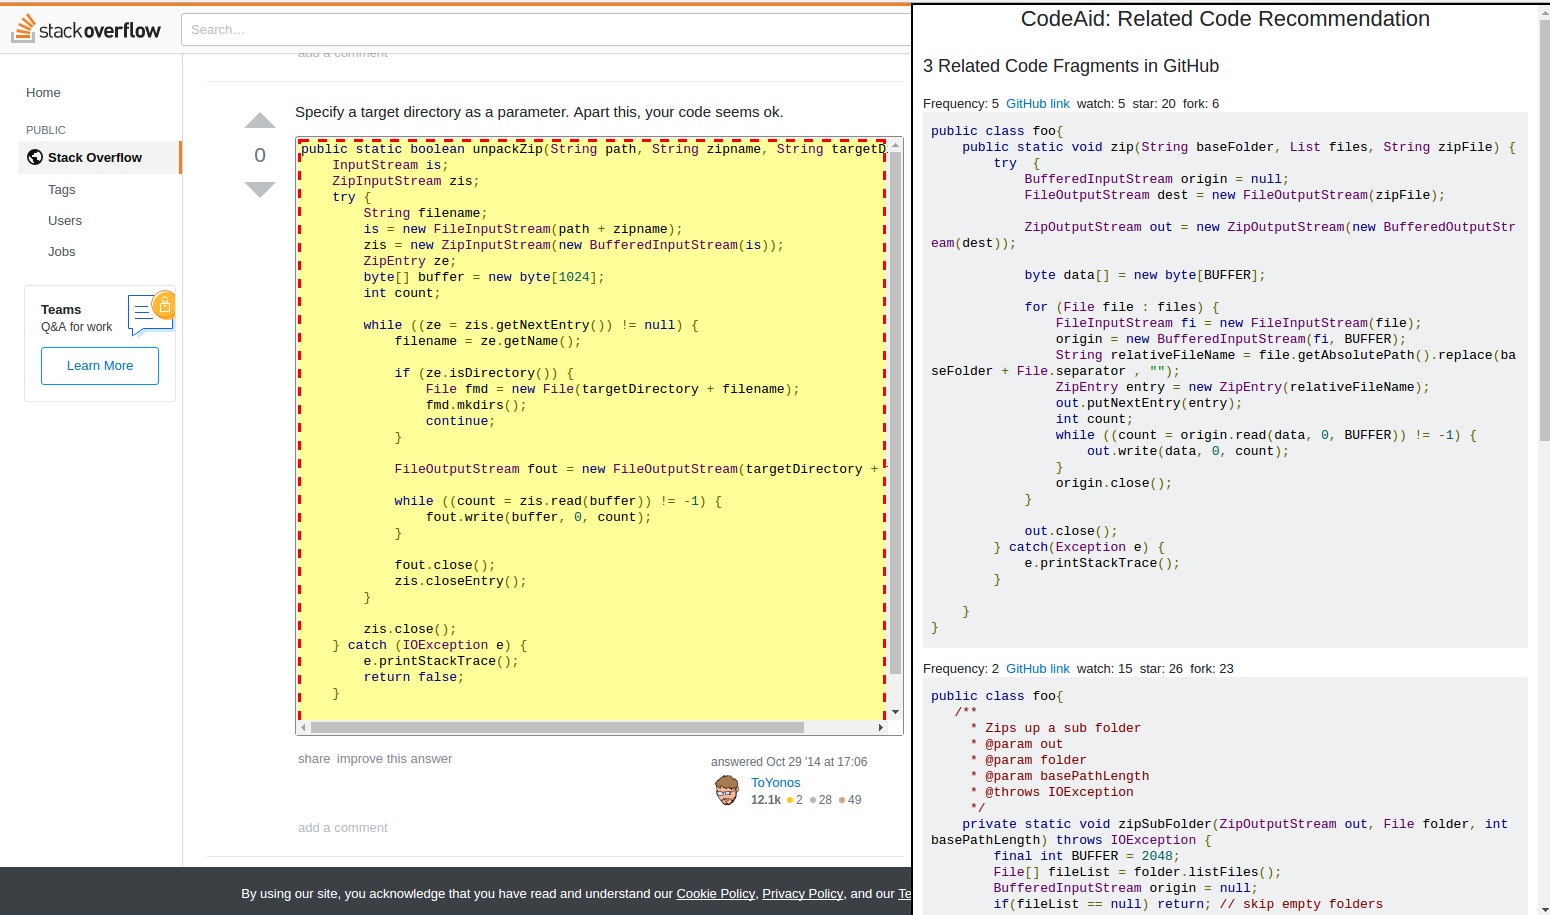
\includegraphics[width=\linewidth]{figures/ui.png}
	\caption{Screenshot of Chrome extension}
	\label{fig:chrome}
\end{figure*}
\section{Related Work}
\label{sec:related}
Various code search techniques have been proposed to discover relevant code components (e.g., functions, code snippets) given a user query. For example, given a keyword query, Portfolio retrieves function definitions and their usages using a combination of a PageRank model and an association model~\cite{mcmillan2011portfolio}. Chan et al.~improve Portfolio by matching the textual similarity between containing nodes in an API usage subgraph with a keyword query~\cite{}. CodeHow also finds code snippets relevant to a natural language query. It explores API documents to identify relationships between query terms and APIs~\cite{lv2015codehow}. Instead of using natural language queries, several techniques automatically recommend relevant code snippets based on contextual information such as types in a target program~\cite{Holmes2005, sahavechaphan2006xsnippet, thummalapenta2007parseweb, ponzanelli2014mining}. CodeGenie is a test-driven code search technique that allows developers to specify desired functionality via test cases and then matches relevant methods and classes with the given test~\cite{lazzarini2009applying}. To more precisely capture search intent, S6 allows developers to express desired functionality using a combination of input-output types, test cases, and keyword descriptions~\cite{reiss2009semantics}.

Code-to-code search tools are most related to our technique among all different kinds of code search techniques. Given a code snippet as input, FaCoY finds semantically similar code snippets in a Stack Overflow dataset by first matching with accompanied natural language descriptions in related posts instead of matching code directly. Unlike FaCoY, several techniques infer an underlying code search pattern from a given code fragment~\cite{zhang2015interactive, MKM:11, meng2013lase, sivaraman2019active}. Sydit generalizes concrete identifiers (e.g., variable names, types, and method calls) in a given code example as an abstract code template and identifies other similar locations via AST-based tree matching~\cite{MKM:11}. Lase uses multiple code examples instead of a single example to better infer the search intent of a user~\cite{meng2013lase}. Critics allows developers to construct an AST-based search pattern from a single example through manual code selection, customization, and parameterization~\cite{zhang2015interactive}. These code-to-code search tools focus on identifying relevant code snippets that are syntactically or semantically similar to a given code snippet. However, since many programming tasks (e.g., password encryption and decryption) require multiple code snippets or functions to work together, none of the existing techniques recommend code snippets that complement a given code snippet to complete desired functionality.



\section{Conclusion}
\label{sec:conclude}

We have presented {\tool}, a code-to-code search technique and tool
that recommends code fragments related to the code query. The
information need that underlies the design of {\tool} is different
from that of traditional code search engines: rather than retrieving
similar code, it retrieves code within the functionality family of the
code query. This broader context allows programmers to be aware of
related code that may be useful when developing their own
functions. {\tool} works by analyzing co-occurrences of code fragments
in very large code bases, such as GitHub projects, and then clustering
those potential matches for a given code query.

We evaluated {\tool} using a large dataset of code queries collected
from Stack Overflow snippets, and a very large code base of Java
projects collected from GitHub. The evaluation shows that {\tool} is
able to find related fragments for 52.4\% of the queries. A closer look at a set of 30
queries shows that {\tool} has a good precision of 75.6\%. This is
a promising result for a new approach to code search. 

One limitation of {\tool} is that the recommendation power of {\tool} strongly correlates with the similarity behavior of the dataset. To retrieve related code fragments, {\tool} requires the query code to have similar counterparts in the search query corpus; it also asks for similar method pairs within search query corpus itself. 

For future work, we may try different user-defined query code base and search code corpus to further evaluate {\tool}. For example the search code corpus can be the code base for a company or previous projects from a user. We may import the tool into a Eclipse plugin and help developers during real life programming process. The use scenario will be, when a user is currently writing a code fragment and uses it as query to search {\tool} plug-in, we will return the ranked list of related code from the company's code base or the user's own projects.

%\section*{References}

\bibliographystyle{plain}

\bibliography{ref}

\end{document}
